{
\setlength{\parindent}{2em}
\chapter{Introduction}\label{cha:intro}
Since the termination of the Space Shuttle program in 2011, the \gls{NASA} has been turning to other countries and private enterprises for the transportation of cargo to orbit and beyond. The \gls{CRS} program is a good example of this : a public-private partnership in which supplies provided by NASA are launched into orbit to the \gls{ISS} by commercial rockets. Of course, the new "Delivery-as-a-Service" paradigm has spawned a lot of commercial interest all around the world. In the United States, the Dream Chaser program is one of those efforts that continue strengthening the ties between public space agencies and the private sector.

\section{The Dream Chaser program}
This thesis' scope is entirely contained within the Dream Chaser project. Therefore, the spacecraft and its design is the main subject. Before expanding into the body of the document, a little background is of course important.
\subsection{History}
Conceptualized in 2004 by SpaceDev, the \gls{DCCS} program was officially kick-started by \gls{SNC} in 2010, following its acquisition of SpaceDev in 2008\cite{online:fikes}. Seeing the potential and future possibilities of the transportation system, NASA then awarded funding for the project as part of their \gls{CCDev} program, furthering the development efforts. As \gls{SNC} started breaking down the spacecraft into several sub-systems, it also started subcontracting their development to other companies. So far, the first flight to the \gls{ISS} is officially scheduled for 2021. However, seeing as the present thesis is taking place in 2020, the launch will most probably be postponed.

\subsection{Features}
The \gls{DCCS} is an unmanned, reusable orbital spaceplane intended for the transportation of both pressurized and unpressurized cargo to and from the \gls{ISS}. It contains many features that make it a very interesting end solution for different kinds of space needs. 

First of all, the system contains a powerful propulsion system made out of a cluster of Orbitec's Vortex engines\cite{online:messier}. This enables self-cruising and orbit correction, instead of being 100\% reliant on the launch provider for exact orbit insertion. Furthermore, this on-board propulsion opens up other possibilities for Dream Chaser deeper than \gls{LEO}, like transporting cargo to the coming Lunar Gateway. 

Secondly, the  spacecraft is partly made reusable by the development of a custom, very resistant airframe by Lockheed Martin. The haul, its wings and landing gear enable \gls{DCCS} to safely land on a runway from \gls{LEO}. With these features, it's of course very easy to compare Dream Chaser to a mini Space Shuttle (see \autoref{fig:dccs_landed}). 
\begin{figure}[H]
	\centering
	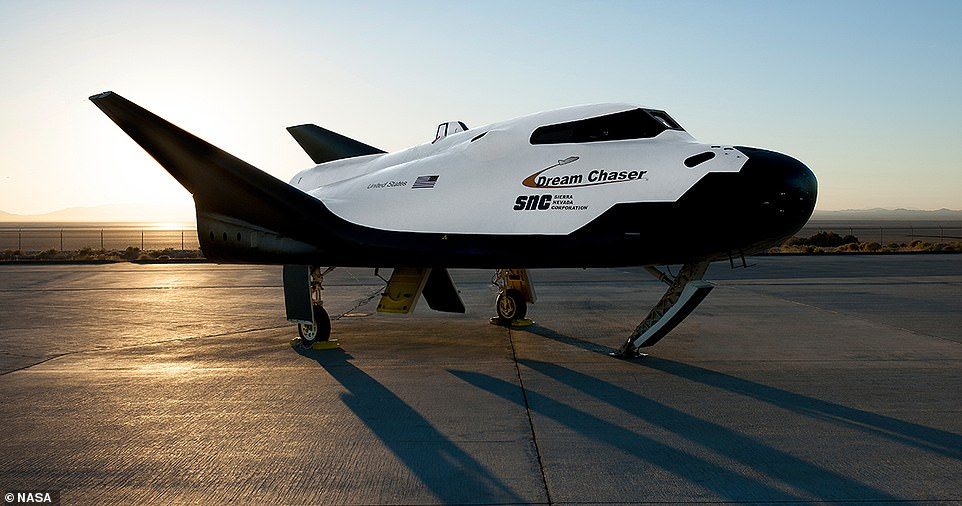
\includegraphics[width=0.9\linewidth, keepaspectratio]{art/dream_chaser_landed.jpg}
	\caption{Dream Chaser on a runway at sunset.}
	\label{fig:dccs_landed}
	\source{Sierra Nevada Corporation \cite{misc:dccs_landed}}
\end{figure}
Finally, its communication subsystem is made of several types of antennas, for encrypted telecommunication with ground stations and the \gls{ISS}. Because docking to the space station is also one the spacecraft's capabilities, a physical communication link is present too. \gls{MDA} has been put in charge of this crucial component's development by \gls{SNC}. 

\section{MDA - Industry partner}
In the emerging Canadian space sector, \gls{MDA} is widely recognized as one of its greatest actors. The Canada-based company, which has offices in Montreal, has already partnered on multiple occasions with the Canadian Space Agency. It's most notable contributions are the design and manufacturing of the Canadarm2 on the \gls{ISS}, as well as the RADARSAT-2 satellite constellation. The current document was made in partnership with \gls{MDA}, in the context of a 6 months thesis-internship in Montreal during which the present project was scoped, planned and executed. The work was officially supervised by Claudio Discepola, Senior member of the Dream Chaser team. 

\section{Background}
With the ever decreasing cost of computing power, functional simulation of components and systems has become an integral part of the testing phase in space design. This approach is thus also taken by \gls{SNC} in the context of Dream Chaser, who requires subcontractors like \gls{MDA} to provide simulators of their respective subsystems alongside the subsystem itself. This is done with the intent of simulating, on multiple fronts, an entire launch or mission, from the reception and handling of telecommands to the behavior of the flight computer mid-mission. 

Once the simulators are all working separately, they are then interfaced together. This results in a compute-intensive platform called the \gls{DCMS}, an important piece in the integration, testing and validation phases of the development. By its virtual nature, the \gls{DCMS} can be ran under different conditions in order to observe the behavior of the spacecraft as a whole in different scenarios. This proves to be of course extremely useful, for example, in the early detection of anomalies or even in the regression testing of software.

Each subcontractor's simulator possesses its own set of requirements, driven by the desired simulation quality and granularity. In that sense, \gls{MDA} is in charge of developing the \gls{BBPSim}, a \gls{SIL} platform for the flight code of the entire communication subsystem, from the antennas to the computing nodes themselves. \gls{BBPSim} acts as some sort of hypervisor, exposing an interface to operating system and hardware utilities to the flight software, itself fundamentally written for an embedded platform. This makes abstraction of the system on which the code is running while keeping all of its functionalities and internal algorithms. As a result, \gls{BBPSim} significantly improves the easiness of interaction with the flight software as while enabling its testing on a Linux machine in a continuous integration pipeline system like Jenkins.

\section{Purpose}
The purpose of this thesis is to design and develop a custom-fit \textit{snapshotting} technique for \gls{BBPSim}. As said previously, the development of the simulator is driven by the requirements derived from its inclusion in the DCMS. The need for a snapshot feature comes from a pair of them, that state that
\begin{enumerate}
	\item \gls{BBPSim} shall have the capability of saving its state, or "context", to non-volatile memory.
	\item \gls{BBPSim} shall be able to restore itself from a state file in non-volatile memory at initialization.
\end{enumerate} 

This snapshotting feature (often called the \textit{Save \& restore} in the document) will be a considerable addition to the \gls{BBPSim} framework. It will add the possibility to exhaustively represent an on-going simulation at a definite time $t$. It is called a snapshot due to its many similarities with virtual machine software like the open-source VirtualBox. In VirtualBox, it is possible for the user to pause, or to "snapshot" a running instance of a virtual machine, to save it into a relatively large file (called state file) and to restore everything back exactly like it was : running programs, graphics card output and general OS state are all recovered.  

Save \& restore has considerable advantages from a testing point of view. For instance, in the context of Dream Chaser, the flight software enters different states depending on the phase of launch the spacecraft is in. The code doesn't have the same behavior during the launch phase than it has when in the docking phase. However, for the software to change state, some sort outside stimuli must be present. There must be some manipulation by an external actor, and this manipulation can last many minutes for each test. Considering there are hundreds of tests, the time for exhaustive regression testing is of course significant. The snapshot feature completely removes that limitation, because it enables the simulator to be instantly started to a previous state without having to interact with the \gls{FSW}. It is possible to shortcut directly to the docking phase without having to go trough simulating the launch phase. 

Furthermore, another benefit of the feature is that it allows the same hypothetical failures to be replayed over and over again. Since a state file can be restored again and again at will, the interaction between all the different subsystems can be analyzed more in-depth. When in the integration phase, potential inter-system faults can be caught earlier and they are easier to reproduce.  

This thesis will start by giving an overview of such a \textit{snapshotting} concept in the context of other software projects. There has been many successful attempts to create this mechanism in academic papers and open-source programs, instances from which inspiration has been drawn. Then the design and implementation of the feature inside \gls{BBPSim} is discussed in details. The general approach in terms of changing the simulator's software to be make it saveable is explained. Beyond these crucial steps, the integration of the work in the existing testing pipeline is also covered, as well as its impact on the testing process at MDA, because it has the potential to improve the past testing procedure.


}